\subsection{Intégration de l'IA multi niveaux}

L'intelligence artificielle actuellement utilisée repose sur les\voc{LLM}. 

Ces modèles produisent du texte. Cela tombe parfaitement bien puisque le langage LaTeX fonctionne exclusivement grâce à du texte. 

Il y a donc plusieurs niveaux sur lesquels l'IA peut agir : 

\begin{MultiColonnes}{2}[colframe=black,boxrule=0.4pt,fonttitle=\bfseries]%
    \tcbitem[title=Debuguer] Sur copie d'un contenu \LaTeX\ la plupart des outils IA actuels peuvent : 
    \begin{itemize}[label=$\bullet$]
        \item Le corriger
        \item Déterminer l'en-tete correspondante
        \item Le modifier en suivant des instructions basiques
    \end{itemize}
    \tcbitem[title=Produire du contenu] Sur base d'un modèle \LaTeX\ et d'une série d'instructions précises, certains modèles peuvent produire du contenu \LaTeX\ de qualité. 
    \tcbitem[title=Recopier du contenu] Sur base d'un modèle \LaTeX\ et d'une série d'instructions précises, certains modèles peuvent reprendre un document pdf ou image pour produire du contenu \LaTeX. 
    \tcbitem[title=Créer des packages] L'IA peut fabriquer des commandes ou environnements qui répondent à vos besoins spécifiques et les intégrer dans vos \acc{documents} ou dans vos \acc{packages}
    \tcbitem[title=Agent formateur] Sur base d'un extrait de documentation, l'IA peut résumer les principales fonctionnalités disponibles et vous fournir celles dont vous avez besoin en lien avec vos demandes. 

    On peut faire produire des rapports ( markdown ou \LaTeX\ ) pour que l'IA nous \acc{forme} à utiliser certaines technologies. 

    C'est de cette manière dont j'ai appris \LaTeX. 
    \tcbitem[title=Agent modérateur] Certains modèles de langage avancés sont capable de jouer le rôle d'agent principal en actionnant divers outils. 
    
    Cela dépasse largement le cadre de cette formation, mais on peut envisager un agent IA qui irait se documenter sur internet, produire quelques diapos avec canvas, produire un genially d'une activité et produire une fiche d'activité \LaTeX\ pour donner les consignes aux élèves dans laquelle figureraient les qrcode. 
\end{MultiColonnes}



\bcattention Les solutions pour intégrer l'IA dans sa démarche de travail nécessitent un abonnement dont les prix vont - actuellement - de $10$\euro{} par mois ( Github Copilot ) à $200$\euro{} par mois ( ChatGPT max ).

La plupart des abonnements \frquote{pro} coûtent environ $20$\euro{} par mois et correspondent aux besoins d'un enseignant qui se forme au \LaTeX. 
Il suffit de choisir un modèle et de l'utiliser avec cette formule. 
\begin{Methode}[Les grands principes]
    L'intégration de l'IA repose sur les principes suivants : 


    \begin{MultiColonnes}{2}[colframe=black,boxrule=0.4pt,fonttitle=\bfseries]%

        \tcbitem[title=Un modèle] Parfois on préfère un \encadrer{modèle rapide}, parfois un \encadrer{modèle de réflexion}, parfois un \encadrer{modèle d'action} et parfois un \encadrer{modèle multimodal} ( images, voix... )

        \tcbitem[title=Un système d'intégration] On peut \encadrer{copier/coller} le code produit par le modèle. On peut également permettre à l'IA de produire son code sur votre ordinateur via un \encadrer{logiciel}.

        \tcbitem[raster multicolumn=2, title=Des prompts] C'est le plus important. Ce prompt doit être : 
        \begin{itemize}[label=$\bullet$]
            \item \encadrer{Cohérent} \hfill Permet une réponse sans bugs et sans oubli.
            \item \encadrer{Fourni en exemples de qualité} \hfill Votre style sera copié.
            \item \encadrer{Structuré - XML / markdown} \hfill L'IA intègrera mieux les informations et en plus grande quantité.
        \end{itemize}
    \end{MultiColonnes}
    \bcattention Les modèles actuels sont limités par leur\voc{fenêtre de contexte}. 

    C'est la taille de leur \acc{mémoire de travail}. Actuellement elle se situe entre $\num{200000}$ et $\num{1000000}$ tokens, ce qui correspond à un livre de $500$ pages.

    Cela paraît beaucoup, mais cette limite est atteinte très rapidement en réalité. 

    \encadrer[green]{Une demande IA par discussion}. 

    Cette limitation rendra vos interactions plus efficaces. Les prompts seront également plus simple, et vous pouvez \acc{masquer du contexte} pour que l'agent se concentre uniquement sur sa tâche. 
\end{Methode}
%\newpage%

\subsection{Protocoles de communication}
\begin{Definition}[Protocole MCP et A2A]
    Un \acc{modèle de langage} produit des \acc{tokens} de texte. 

    Un \acc{modèle de langage} ayant accès à des outils numériques est appelé un\voc{agent}.

    Les agents produisent des tokens qui peuvent leur servir à communiquer avec : 

    \begin{MultiColonnes}{2}
        \tcbitem $\bullet$ Des applications $\rightarrow$ protocole \encadrer{MCP}. 
        \tcbitem $\bullet$ D'autres agents IA $\rightarrow$ protocole \encadrer{A2A}. 
    \end{MultiColonnes}

    Ces deux protocoles sont basés sur des \acc{requêtes} : l'agent formule une requête et le serveur lui renvoie un signal. \\

    Pour l'usage de LaTeX avec un agent IA, nous nous intéresseront à l'usage du protocole MCP.

    Le protocole A2A sera utilisé dans des applications plus ambitieuses pour \acc{synchroniser des agents}. 

    Ce protocole \acc{étend les possibilités du précédent} aux communications \acc{asynchrones}.
\end{Definition}
\begin{Exemple}[Architecture d'agent avec MCP]
    \begin{tcolorbox}[
        title=Mode agentique MCP seulement,
        colback=blue!5!white,
        colframe=blue!50!black,
        width=\textwidth,
        boxrule=0.4pt,
        left=2pt,right=2pt,top=2pt,bottom=2pt
    ]
        \begin{tcbraster}[
            raster columns=5,
            raster equal height=rows,
            raster column skip=1cm,
            raster row skip=8pt
        ]
            % utilisateur
            \begin{tcolorbox}[
                blankest,
                halign=center,
                valign=center,
                height=3cm
            ]
                \tikzmark{mcp-user}utilisateur\tikzmark{mcp-user-end}
            \end{tcolorbox}
            % agent
            \begin{tcolorbox}[
                blankest,
                halign=center,
                valign=center
            ]
                \tikzmark{mcp-agent}agent\tikzmark{mcp-agent-end}
            \end{tcolorbox}            
            % Colonne outil 1
            \begin{tcolorbox}[
                blankest
            ]
                \begin{tcbraster}[
                    raster columns=1,
                    raster row skip=3pt
                ]
                    \begin{tcolorbox}[
                        blankest,
                        halign=center,
                        height=0.8cm
                    ]
                        \tikzmark{mcp-outil1-top}outil 1
                    \end{tcolorbox}
                    \begin{tcolorbox}[
                        blankest,
                        halign=center
                    ]
                        \parbox{3cm}{\centering \tikzmark{mcp-analyse1}analyse et\\poursuite de la\\tâche}\tikzmark{mcp-analyse1-end}
                    \end{tcolorbox}
                \end{tcbraster}
            \end{tcolorbox}
            % Colonne outil 2
            \begin{tcolorbox}[
                blankest
            ]
                \begin{tcbraster}[
                    raster columns=1,
                    raster row skip=3pt
                ]
                    \begin{tcolorbox}[
                        blankest,
                        halign=center,
                        height=0.8cm
                    ]
                        \tikzmark{mcp-outil2-top}outil 2
                    \end{tcolorbox}
                    \begin{tcolorbox}[
                        blankest,
                        halign=center
                    ]
                        \parbox{3cm}{\centering \tikzmark{mcp-analyse2}analyse et\\poursuite de la\\tâche}\tikzmark{mcp-analyse2-end}
                    \end{tcolorbox}
                \end{tcbraster}
            \end{tcolorbox}            
            % fin
            \begin{tcolorbox}[
                blankest,
                halign=center,
                valign=center
            ]
                \tikzmark{mcp-fin}Fin de la tâche
            \end{tcolorbox}
        \end{tcbraster}
        
        % Flèches
        \tikz[remember picture,overlay] {
            % utilisateur → agent
            \draw[->,thick] ([xshift=3pt]pic cs:mcp-user-end) -- ([xshift=-3pt]pic cs:mcp-agent);
            % agent → outil 1 (haut)
            \draw[->,thick] ([xshift=3pt]pic cs:mcp-agent-end) to[out=0,in=180] ([xshift=-3pt,yshift=3pt]pic cs:mcp-outil1-top);
            % outil 1 (analyse) → outil 2 (haut)
            \draw[->,thick] ([xshift=3pt]pic cs:mcp-analyse1-end) to[out=0,in=180] ([xshift=-3pt,yshift=3pt]pic cs:mcp-outil2-top);
            % outil 2 (analyse) → fin
            \draw[->,thick] ([xshift=3pt]pic cs:mcp-analyse2-end) -- ([xshift=-3pt]pic cs:mcp-fin);
        }
    \end{tcolorbox}
\end{Exemple}
\begin{Exemple}[Architecture d'agent avec A2A]
    \begin{tcolorbox}[
        title=Mode agentique A2A,
        colback=green!5!white,
        colframe=green!50!black,
        width=\textwidth,
        boxrule=0.4pt,
        left=2pt,right=2pt,top=2pt,bottom=2pt
    ]
        \begin{tcbraster}[
            raster columns=5,
            raster equal height=rows,
            raster column skip=1cm,
            raster row skip=8pt
        ]
            % utilisateur
            \begin{tcolorbox}[
                blankest,
                halign=center,
                valign=center,
                height=4cm
            ]
                \tikzmark{a2a-user}utilisateur\tikzmark{a2a-user-end}
            \end{tcolorbox}
            % agent
            \begin{tcolorbox}[
                blankest,
                halign=center,
                valign=center
            ]
                \tikzmark{a2a-agent}agent\tikzmark{a2a-agent-end}
            \end{tcolorbox}            
            % Colonne opérateurs
            \begin{tcolorbox}[
                blankest
            ]
                \begin{tcbraster}[
                    raster columns=1,
                    raster row skip=2pt
                ]
                    \begin{tcolorbox}[
                        blankest,
                        halign=center,
                        height=1cm
                    ]
                        \tikzmark{a2a-op1}opérateur IA 1\tikzmark{a2a-op1-end}
                    \end{tcolorbox}
                    \begin{tcolorbox}[
                        blankest,
                        halign=center,
                        height=1cm
                    ]
                        \tikzmark{a2a-op2}opérateur IA 2\tikzmark{a2a-op2-end}
                    \end{tcolorbox}
                    \begin{tcolorbox}[
                        blankest,
                        halign=center,
                        height=1cm
                    ]
                        \tikzmark{a2a-op3}opérateur IA 3\tikzmark{a2a-op3-end}
                    \end{tcolorbox}
                \end{tcbraster}
            \end{tcolorbox}
            % analyse
            \begin{tcolorbox}[
                blankest,
                halign=center,
                valign=center
            ]
                \tikzmark{a2a-analyse}\parbox{3cm}{\centering analyse et traitement des\\réponses\\multiples}\tikzmark{a2a-analyse-end}
            \end{tcolorbox}
            % fin
            \begin{tcolorbox}[
                blankest,
                halign=center,
                valign=center
            ]
                \tikzmark{a2a-fin}Fin de la tâche
            \end{tcolorbox}
        \end{tcbraster}        
        % Flèches
        \tikz[remember picture,overlay] {
            % utilisateur → agent
            \draw[->,thick] ([xshift=3pt]pic cs:a2a-user-end) -- ([xshift=-3pt]pic cs:a2a-agent);
            % agent → opérateurs (divergence)
            \draw[->,thick] ([xshift=3pt]pic cs:a2a-agent-end) to[out=0,in=180] ([xshift=-3pt]pic cs:a2a-op1);
            \draw[->,thick] ([xshift=3pt]pic cs:a2a-agent-end) to[out=0,in=180] ([xshift=-3pt]pic cs:a2a-op2);
            \draw[->,thick] ([xshift=3pt]pic cs:a2a-agent-end) to[out=0,in=180] ([xshift=-3pt]pic cs:a2a-op3);
            % opérateurs → analyse (convergence)
            \draw[->,thick] ([xshift=6pt]pic cs:a2a-op1-end) to[out=0,in=180] ([xshift=0pt,yshift=10pt]pic cs:a2a-analyse);
            \draw[->,thick] ([xshift=6pt]pic cs:a2a-op2-end) to[out=0,in=180] ([xshift=0pt]pic cs:a2a-analyse);
            \draw[->,thick] ([xshift=6pt]pic cs:a2a-op3-end) to[out=0,in=180] ([xshift=0pt,yshift=-10pt]pic cs:a2a-analyse);
            % analyse → fin
            \draw[->,thick] ([xshift=3pt]pic cs:a2a-analyse-end) -- ([xshift=-3pt]pic cs:a2a-fin);
        }
        \vspace{-1.5cm}\begin{center}
            \textit{chaque opérateur peut utiliser des MCP}
        \end{center}
    \end{tcolorbox}
\end{Exemple}
\subsection{En pratique}
\begin{Aide}[Mettre en place Claude]

    \begin{MultiColonnes}{5}
        \tcbitem[raster multicolumn=2] L'entreprise Anthropic et son modèle \acc{Claude 4-opus} sont à l'origine du \acc{protocole MCP} : \acc{Model Context Protocol}.
        
        Cela permet aux agents d'utiliser \acc{n'importe quel outil numérique}. 
    
        \tcbitem[raster multicolumn=3] Entre autres : 
    \begin{itemize}[label=$\bullet$]
        \item Votre système de fichiers
        \item Aller sur internet
        \item Utiliser n'importe quel outil externe qui propose des fonctionnalités publiques destinées aux agents IA ( canvas par exemple... )
    \end{itemize}
    \end{MultiColonnes}
    

    \begin{MultiColonnes}{5}
        \tcbitem[raster multicolumn=3] J'utilise au quotidien ce modèle d'IA via\vocnoindexref{https://claude.ai/download}{l'application locale}. \\
    
    Je propose mes \acc{prompts} comme base officielle pour utiliser \acc{bfcours} avec Claude.

    Cela lui permet de préparer les documents avec mes exigences de qualité.
    \tcbitem[raster multicolumn=2,colframe=\itemBaseColor,title=Prompts de bfcours, boxrule=0.4pt,fonttitle=\bfseries,halign=left] \dirtree{%
        .1 \bfseries fichiers\_de\_la\_formation/.
        .2 ressources/.
        .3 \textcolor{red!75!white}{prompts\_claude\_ai/}.
        .3 \textcolor{blue!75!white}{fichiers\_exemples\_a\_donner/}.
        .3 \textcolor{purple!75!white}{claude\_config\_mcp.json}.
    }
    \end{MultiColonnes}
    L'intervention humaine de modification est bien sûr toujours possible. 
    
    L'agent codeur est également à même de modifier par la suite le code qu'il a créé.

    \begin{tcbenumerate}[2]
        \tcbitem Création d'un nouveau projet. Cela revient à créer un \acc{agent}. 

        \vspace{-0.3cm}\begin{center}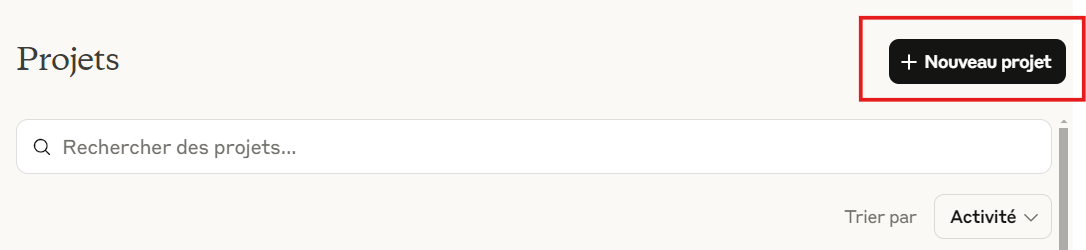
\includegraphics[width=0.75\textwidth]{images/Claude_setup_projects/new-project.png}\end{center}
        \tcbitem Décrire l'agent ( pour l'utilisateur seulement ). 

        \vspace{-0.3cm}\begin{center}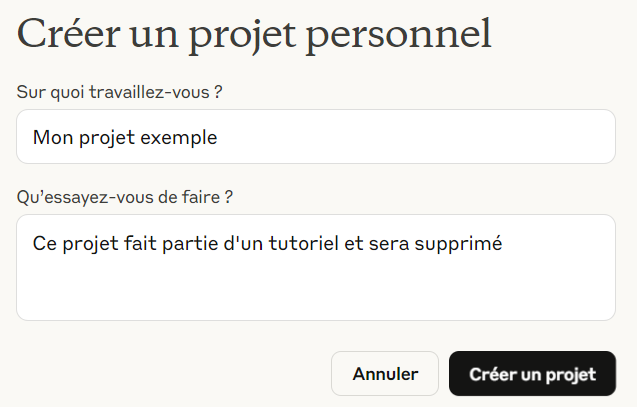
\includegraphics[width=0.55\textwidth]{images/Claude_setup_projects/base-setup.png}\end{center}
        \tcbitem Donner ses instructions. 

        \vspace{-0.3cm}\begin{center}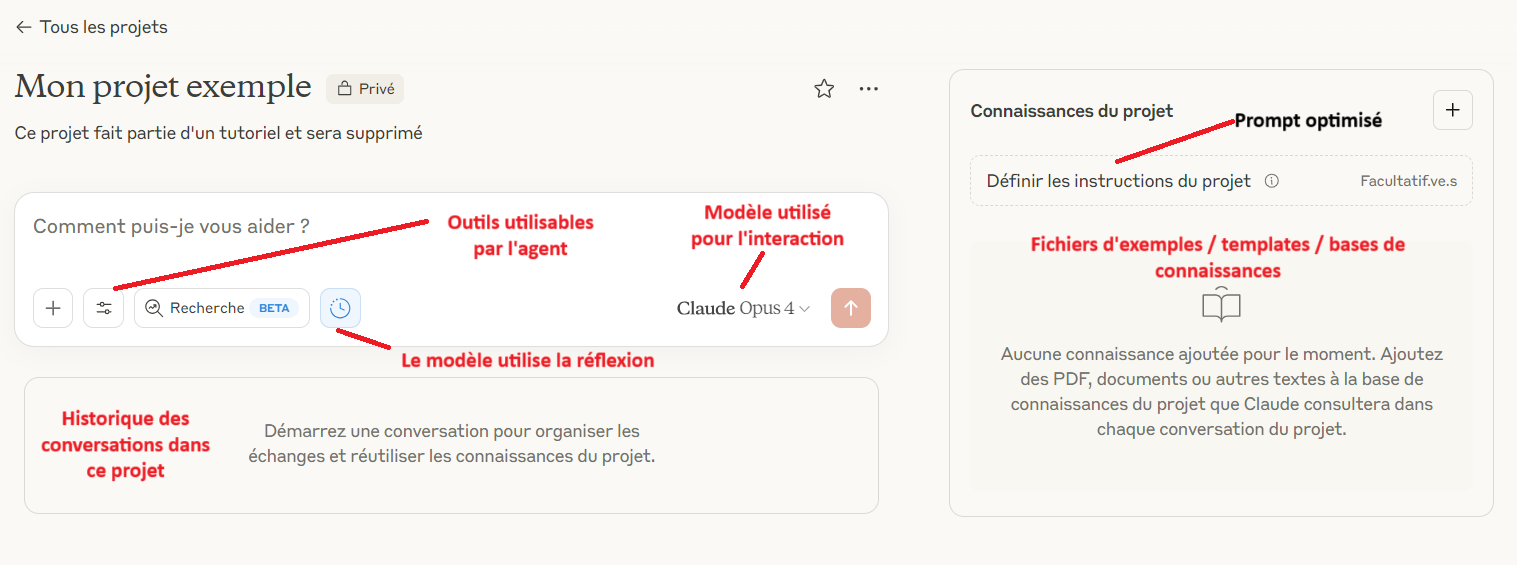
\includegraphics[width=0.95\textwidth]{images/Claude_setup_projects/complete-setup.png}\end{center}

        \tcbitem Votre agent est utilisable dans une \acc{nouvelle conversation}. 

        \vspace{-0.3cm}\begin{center}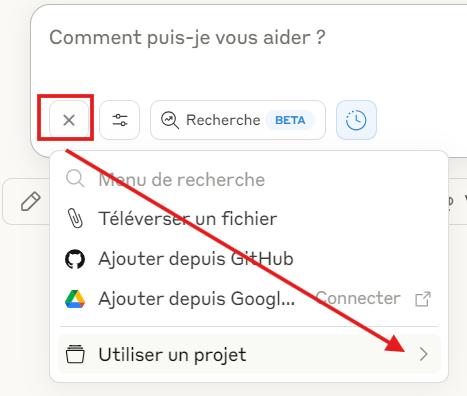
\includegraphics[width=0.55\textwidth]{images/Claude_setup_projects/use-setup.png}\end{center}
    \end{tcbenumerate}

    \begin{bfbox}{Mettre en place les MCP}
    \begin{tcbenumerate}[2]
        \tcbitem Accéder aux paramètres. 
        
        \vspace{-0.3cm}\begin{center}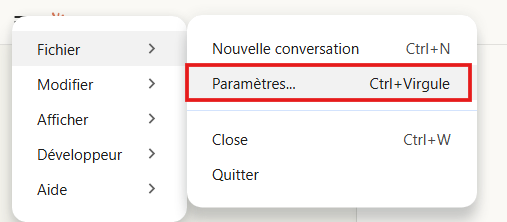
\includegraphics[width=0.55\textwidth]{images/Claude-setup-mcp/1.png}\end{center}
        \tcbitem Activer et accéder aux paramètres développeurs. 
        
        \vspace{-0.3cm}\begin{center}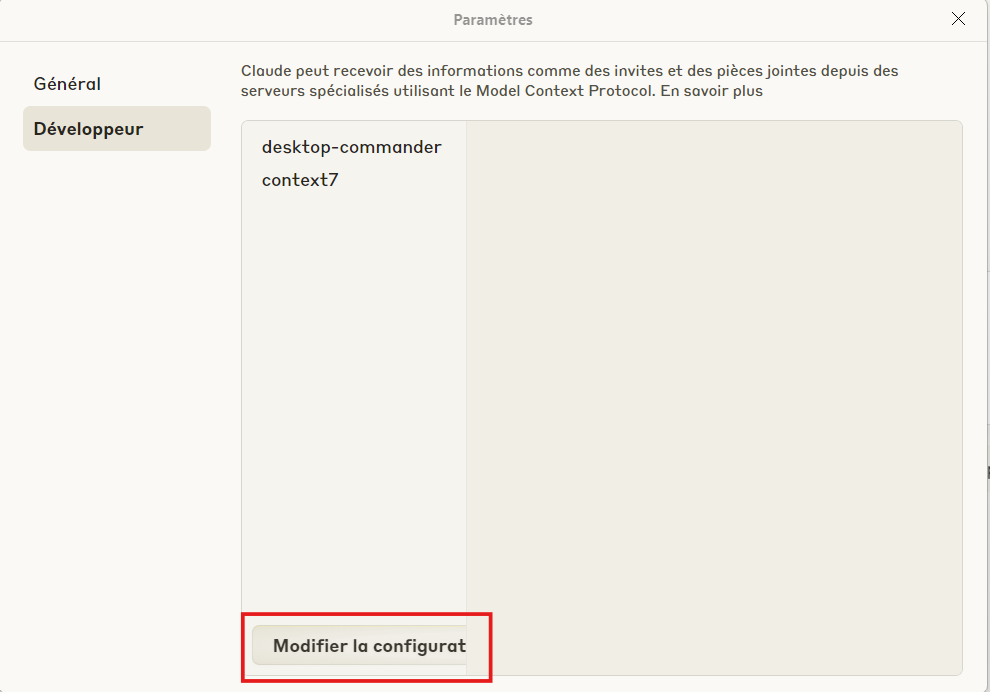
\includegraphics[width=0.55\textwidth]{images/Claude-setup-mcp/2.png}\end{center}
        \tcbitem Modifier le json des serveurs MCP comme donné dans les \acc{fichiers de la formation}.

        \vspace{-0.3cm}\begin{center}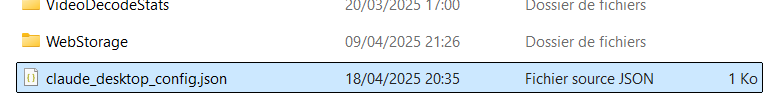
\includegraphics[width=0.55\textwidth]{images/Claude-setup-mcp/3.png}\end{center}

        \tcbitem Votre agent peut utiliser votre système de fichiers. 
    \end{tcbenumerate}
    \end{bfbox}
\end{Aide}

\begin{Aide}[Utiliser Windsurf ou Cursor]
    Ce sont des IDE comme VScode qui intègrent naturellement l'IA dans leur fonctionnement. Soutenus par de grandes entreprises une grande communauté de développeurs.

    On peut utiliser le même \acc{prompt system} que celui donné dans l'aide précédente. 
\end{Aide}

\begin{Aide}[Github Copilot]
    Ce modèle s'intègre bien dans VSCode et permet de la génération de code \LaTeX\ avec des suggestions. 

    Je ne l'utilise pas, mais c'est une solution plus discrète adaptée à ceux qui souhaitent rester maître du code écrit. 
    
    L'IA intervient pour \acc{suggérer} des modifications \acc{en contexte}. Il s'agit d'une alternative \acc{peu coûteuse}.
\end{Aide}


\subsection{Guidelines pour prompts structurés (2025)}

\begin{Definition}[Prompts structurés modernes]
    Les \voc{prompts structurés} représentent l'évolution des techniques de prompt engineering en 2025, combinant la précision du \acc{XML} pour la structure logique avec la lisibilité du \acc{Markdown} pour le contenu.
    
    Cette approche permet d'obtenir des réponses plus fiables et cohérentes des modèles de langage comme Claude d'Anthropic.
\end{Definition}

\begin{Methode}[Structure XML + Markdown]
    \begin{tcbraster}[raster columns=2,raster equal height=rows]
        \begin{tcolorbox}[title=Principe fondamental]
            \begin{itemize}[label=$\bullet$,itemsep=1.3em,leftmargin=*]
                \item \acc{XML} pour la \voc{structure logique}
                \item \acc{Markdown} pour le \voc{formatage du contenu}
                \item \voc{Balises sémantiques} descriptives
            \end{itemize}
        \end{tcolorbox}
        \begin{tcolorbox}[title=Exemple de base, colback=gray!5, colframe=gray!50]
            \ttfamily\small
            \xmltag{instructions}\\
            \hspace{1em}\#\# Tâche principale\\
            \hspace{1em}- Analyser le document\\
            \hspace{1em}- Extraire les points clés\\
            \hspace{1em}- **Formater** la sortie\\
            \xmlctag{instructions}
        \end{tcolorbox}
    \end{tcbraster}
\end{Methode}
\begin{Methode}[Ordre optimal des sections]
    L'ordre des sections dans un prompt structuré suit une progression logique du général au spécifique :
    
    \begin{tcbenumerate}[2]
        \tcbitem \xmltag{system_role} -- Qui est l'agent
        \tcbitem \xmltag{context} -- Situation et environnement  
        \tcbitem \xmltag{data} -- Données de référence
        \tcbitem \xmltag{rules} -- Règles et contraintes
        \tcbitem \xmltag{examples} -- Exemples few-shot
        \tcbitem \xmltag{instructions} -- Actions à effectuer
        \tcbitem \xmltag{output_format} -- Format de sortie
        \tcbitem \xmltag{critical_reminders} -- Points essentiels
    \end{tcbenumerate}
\end{Methode}

\begin{Exemple}[Prompt pour agent créateur de cartes \frquote{J'ai / Qui a}]
    Voici un exemple de prompt pour un agent spécialisé dans la création de cartes mathématiques :

    \begin{MultiColonnes}{2}
        \tcbitem \ttfamily\small
        \xmlbox{?xml version="1.0" encoding="UTF-8"?}\\[0.5em]
        \xmltag{agent_prompt}\\
        \hspace{1em}\xmltag{system_role}\\
        \hspace{2em}Expert LaTeX en création de jeux\\
        \hspace{2em}mathématiques pédagogiques\\
        \hspace{2em}Spécialiste tcolorbox et bfcours\\
        \hspace{1em}\xmlctag{system_role}\\[0.5em]
        \hspace{1em}\xmltag{context}\\
        \hspace{2em}\xmltag{level}Collège 4ème\xmlctag{level}\\
        \hspace{2em}\xmltag{topic}Calcul littéral\xmlctag{topic}\\
        \hspace{2em}\xmltag{cards_count}24\xmlctag{cards_count}\\
        \hspace{2em}\xmltag{objective}Jeu de révision\xmlctag{objective}\\
        \hspace{1em}\xmlctag{context}\\[0.5em]
        
        \tcbitem \ttfamily\small 
        \hspace{1em}\xmltag{instructions}\\
        \hspace{2em}\#\# Créer un jeu complet avec :\\
        \hspace{2em}1. **Cartes bouclées** (dernière $\rightarrow$ première)\\
        \hspace{2em}2. **Progression** de difficulté\\
        \hspace{2em}3. **Variété** des expressions\\[0.5em]
        \hspace{2em}\#\# Contraintes techniques :\\
        \hspace{2em}- Utiliser \textbackslash{}definecolor\{cardcolor\}\\
        \hspace{2em}- Format A4 avec 8 cartes/page\\
        \hspace{2em}- Police lisible (12pt minimum)\\
        \hspace{1em}\xmlctag{instructions}\\[0.5em]
        \hspace{1em}\xmltag{card_structure}\\
        \hspace{2em}\xmltag{front}J'ai : [expression]\xmlctag{front}\\
        \hspace{2em}\xmltag{back}Qui a : [question]\xmlctag{back}\\
        \hspace{1em}\xmlctag{card_structure}
    \end{MultiColonnes}
\end{Exemple}
\vspace{-0.5cm}\begin{Remarque}[Anti-patterns à éviter]
    \vspace{-0.5cm}\begin{Colonnes}[2]%[raster columns=2, raster equal height]
        \begin{tcolorbox}[title={\textcolor{red!75!white}{\textcolor{red}{\faTimes} À éviter}}, colback=red!5]
            \begin{itemize}[label=$\times$]
                \item Instructions négatives excessives (\frquote{Ne fais pas...})
                \item Balises XML invalides ou mal fermées
                \item Mélange contexte/instructions
                \item Exemples incohérents en format
                \item Instructions incohérentes
            \end{itemize}
        \end{tcolorbox}
        \begin{tcolorbox}[title={\textcolor{green!70!black}{$\checkmark$ Bonnes pratiques}}, colback=green!5]
            \begin{itemize}[label=$\checkmark$]
                \item Instructions positives claires
                \item Structure XML valide et cohérente
                \item Séparation nette des sections
                \item Exemples uniformes
                \item Concision, précision et cohérence
            \end{itemize}
        \end{tcolorbox}
    \end{Colonnes}
\end{Remarque}
\begin{Methode}[Techniques avancées]
    \begin{MultiColonnes}{2}
        \tcbitem \textbf{Chain of Thought} 

        Technique permettant de décomposer le raisonnement :
        
        \begin{tcolorbox}[colback=gray!5, colframe=gray!50]
            \ttfamily\small
            \xmltag{thinking_process}\\
            \hspace{1em}1. D'abord, analyser...\\
            \hspace{1em}2. Ensuite, vérifier...\\
            \hspace{1em}3. Finalement, produire...\\
            \xmlctag{thinking_process}
        \end{tcolorbox}
        \tcbitem \textbf{Scratchpad} 

        Pour les documents longs, utiliser un bloc-notes :

        \vfill
        \begin{tcolorbox}[colback=gray!5, colframe=gray!50]
            \ttfamily\small
            \xmltag{scratchpad}\\
            \hspace{1em}Points clés à retenir :\\
            \hspace{1em}- Information critique 1\\
            \hspace{1em}- Donnée importante 2\\
            \xmlctag{scratchpad}
        \end{tcolorbox}
    \end{MultiColonnes}
    \begin{tcolorbox}[title=Scratchpad permanent :,colback=gray!5, colframe=gray!50]
        \ttfamily\small
        \xmltag{scratchpad}\\
        \hspace{1em}Utilise le fichier \displayFilePath{mon\_repertoire\_IA/AI\_NOTES.xml} pour :\\
        \hspace{1em}- Noter ton plan d'action\\
        \hspace{1em}- Tenir à jour les étapes effectuées au fur et à mesure.\\
        \xmlctag{scratchpad}
    \end{tcolorbox}
    \encadrer[purple]{Cette dernière méthode est extrêmement efficace et permet aux agents de se succéder de façon fluide.}
\end{Methode}

\begin{Methode}[Prompt optimisé]
    Adapter la structure selon le type de tâche :
    
    \begin{MultiColonnes}{3}[colframe=\itemBaseColor,boxrule=0.4pt]
        \tcbitem[title=Pour du code,halign=left] 
        \begin{itemize}[label=$\bullet$,leftmargin=*]
            \item Structure de fichiers attendue
            \item Conventions de nommage
            \item Exemples d'entrée/sortie
        \end{itemize}
        \tcbitem[title=Pour des documents] 
        \begin{itemize}[label=$\bullet$]
            \item Templates de structure
            \item Styles d'écriture
            \item Ton et registre
        \end{itemize}
        \tcbitem[title=Pour des analyses] 
        \begin{itemize}[label=$\bullet$]
            \item Critères d'évaluation
            \item Métriques à calculer
            \item Format de rapport
        \end{itemize}
    \end{MultiColonnes}

    Pour un agent spécialisé en \LaTeX\ avec \acc{bfcours}, voici la structure optimale :
        \dirtree{%
            .1 \xmltag{latex_agent_prompt}.
            .2 \xmltag{system_role} \DTcomment{\color{green!75!black}Expert LaTeX/bfcours}.
            .2 \xmltag{context} \DTcomment{\color{green!75!black}Environnement pédagogique}.
            .2 \xmltag{bfcours_conventions}.
            .3 \xmltag{environments} \DTcomment{\color{green!75!black}Definition, Exemple, etc.}.
            .3 \xmltag{commands} \DTcomment{\color{green!75!black}\textbackslash voc, \textbackslash acc, etc.}.
            .3 \xmltag{layout} \DTcomment{\color{green!75!black}MultiColonnes, tcbraster}.
            .2 \xmltag{quality_requirements}.
            .3 \xmltag{imperative_rules} \DTcomment{\color{green!75!black}Règles strictes}.
            .3 \xmltag{design_principles} \DTcomment{\color{green!75!black}Principes de design}.
            .2 \xmltag{workflow_instructions}.\DTcomment{\color{green!75!black}Patterns de travail / chaîne de pensée}.
            .2 \xmltag{critical_reminders}.\DTcomment{\color{green!75!black}Points clés à respecter ( synthétique )}.
        }
\end{Methode}
\begin{bfbox}{Processus d'itération}
    \begin{tcbenumerate}[2]
        \tcbitem \textbf{Tester} avec des cas limites variés
        \tcbitem \textbf{Analyser} les échecs et réussites
        \tcbitem \textbf{Enrichir progressivement} la structure et les instructions
        \tcbitem \textbf{Affiner} le prompt
        \tcbitem \textbf{Conserver} une bibliothèque de prompts testés
        \tcbitem \textbf{Partager} les agents efficaces découverts
    \end{tcbenumerate}
    %\vspace{-0.6cm}
    \begin{center}
        \acc{Règle d'or :}
    \encadrer[\itemBaseColor]{Un prompt bien structuré}
            {\huge =}
            \encadrer[\itemBaseColor]{Moins de corrections} 
            {\huge +} 
            \encadrer[\itemBaseColor]{Meilleure productivité}\\

        \encadrer[cyan]{\frquote{La structure parfaite émerge de l'expérimentation continue.}}
    \end{center}

    
\end{bfbox}